\newpage %--Удалить, когда будет не нужно, я добавил его чтобы не было лажи с форматированием
\lecture{3}{15 April}{\dag}
\subsection{Подсчет углов в графе}

\begin{figure}[h!]
    \begin{minipage}{0.7\textwidth}
        Рассмотрим \textbf{ориентированный} граф без кратных ребер и петель.
        
        Назовем \textit{треугольником} упорядоченную тройку $ (x, y, z)$, если это цикл из трех вершин. \textit{Углом} назовем тройку  $ (x, y, z)$, если есть ребра  $ xy$ и $xz$, при этом  $ y $ может совпадать  $ z$.
        
        \textbf{Чего в графе больше: углов или треугольников?}
    \end{minipage}
	\begin{minipage}{0.25\textwidth}
		\center{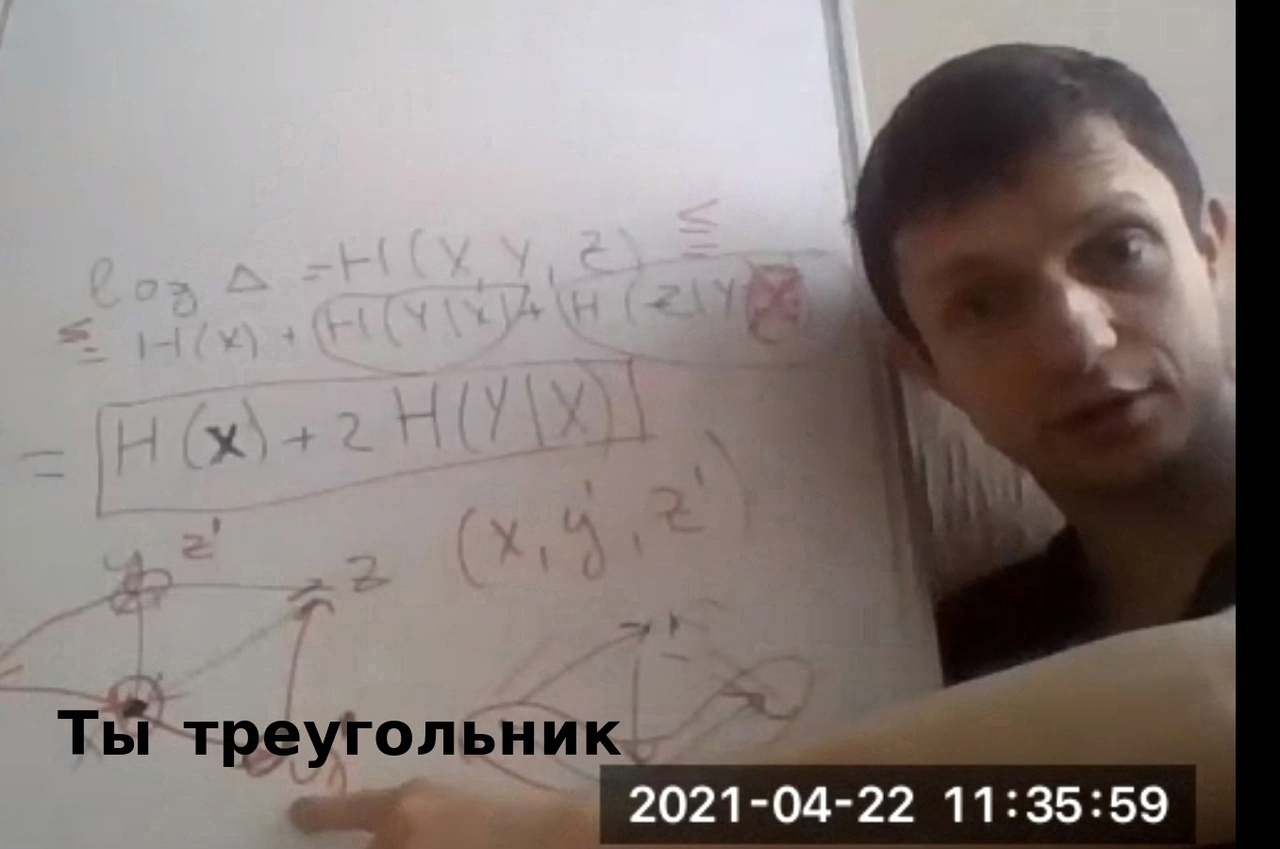
\includegraphics[width=\textwidth]{figures/you_are_triangle.jpg}}
	\end{minipage}
\end{figure}

\begin{note}
	Каждое ребро тоже угол, например, $ (x, y, y)$.
\end{note}
\begin{note}
    Треугольником мы называем именно упорядоченную тройку вершин, которые соединены ребрами между собой. Поэтому просто треугольник даёт вклад равный 3 <<упорядоченным>> треугольникам.
\end{note}
\begin{thm}
    Число углов в графе всегда больше или равно числа треугольников.
\end{thm}
\begin{proof}
 	Пусть случайная величина $ \alpha = (X, Y, Z)$ равна случайному треугольнику, где $ X, Y, Z$ --- с.в., соответствующие первой, второй и третьей вершине треугольника в равномерном распределении на треугольниках. 

	Так как распределение количества треугольников равномерно,
	\begin{align*}
		\log (\# \Delta)& = H(X, Y, Z)  = \\
					  &= H(X) + H(Y \mid  X) + H(Z \mid  Y, X) \le \tag{Chain rule}  \\
					  & \le  H(X) + H(Y \mid X) + H(Z \mid Y) = \tag{циклический сдвиг в треугольнике} \\
		 & = H(X) + 2 H(Y \mid X)
	\end{align*}
Найдем какое-то распределение на углах, энтропия которого хотя бы $ H(X) + 2H(Y \mid X)$, тогда эта сумма будет не более  $  \log (\# \angle)) $.
	% с картинкой будет лучше?

	Пусть мы выбрали случайный треугольник $ (x, y, z)$. Оставим $ x$ и выберем для него случайный треугольник с $ x$ и возьмем из него следующую за $ x$ вершину $ y'$. Повторяем эту операцию еще раз для $ x$ и находим  $ z'$. Тогда $ (x,  y', z')$ --- угол.
	\begin{align*}
		H(x, y', z') & = H(x) + H(y' \mid x) + H(z' \mid x, y') = \tag{Так как $ y'$ и  $ z'$ независимы при выбранном  $ x$}  \\
					 & =H(x) + H(y'\mid x) + H(z' \mid x) = \tag{Выбор аналогичный} \\
					 & = H(x) + 2 H(y' \mid x)
	\end{align*}
	$ H(x)$ здесь совпадает с  $ H(x) $ выше, так как мы выбираем треугольник и вершину аналогично.

	$ y'$ выбирается при фиксированном  $ x$ также, как и выше (выбрали случайный треугольник и в нем вершиной после $ x$ будет  $ y'$).

	Таким образом, мы нашли какое-то распределение на углах с такой же энтропией, следовательно, углов не меньше, чем треугольников.
\end{proof}



\chapter{Теория кодирования}
\begin{defn}[Код]
	Будем называть \selectedFont{кодом} функцию $ C \colon \Sigma = \{a_1, \ldots , a_n\} \to \{0, 1\}^{*}$, сопоставляющую буквам некоторого алфавита кодовые слова.

	Если любое сообщение, полученное применением кода $ C$, однозначно декодируется, то такой код будем называть \selectedFont{однозначно декодируемым}.
\end{defn}

\section{Префиксные коды}
\begin{defn}[]
	Код называется \selectedFont{префиксным}, если никакое кодовое слово не является префиксом другого кодового слова. 
\end{defn}
\begin{note}
    Очевидно, из этого следует однозначная декодируемость.
\end{note}

\begin{thm}\label{thm:exists_code}
    Пусть набор целых чисел $  l_1, \ldots , l_n$ удовлетворяет неравенству
	\[
	\sum_{i=1}^{n} 2^{-l_i} \le 1
	.\] 
	Тогда существует префиксный код с кодовыми словами $  c_1, \ldots , c_n$, где $ \lvert c_i \rvert  \le l_i$.
\end{thm}
\begin{proof}
    Индукция по $ n$.
	\begin{itemize}
		\item База: $ n = 1$. Очевидно.
		\item Переход: $ n \to  n+1$. Пусть нам даны числа $  l_1, \ldots , l_{n+1}$.

			\begin{itemize}
				\item Если среди них есть два одинаковых, $  l_1 = l_2$, заменим их на одно $ l = l_1 - 1$, чтобы сохранилась сумма обратных степеней двойки. Теперь можем применить предположение для $ n$ и найти префиксный код со словами $c, c_3, \ldots , c_{n+1}$. Заменим слово $ c$ на $ \overline{c0}$ и $\overline{c1}$, которые будут соответствовать $  l_1$ и $  l_2$. 
				\item Если все различны, то можем выбрать слова длины $  l_1, l_2, \ldots , l_n$ из слов вида $ 0, 10, 110, \ldots $. Этот код будет префиксным, так как у всех разное число единиц перед нулем.
			\end{itemize}
	\end{itemize}
\end{proof}

\begin{thm}[Неравенство Крафта-Макмиллана]\label{thm:km}
    Для любого однозначно декодируемого кода с кодовыми словами $  c_1, \ldots , c_n$ выполнено неравенство
	\[
	\sum_{i=1}^{n} 2^{-\lvert c_i \rvert } \le 1
	.\] 
\end{thm}
\begin{proof}
	Построим многочлен для всех слов длины $ L$. 

	Для этого воспользуемся следующей идеей.

	Строка длины $L$ переходит в конкатенацию кодовых слов для каждого символа исходной строки.
	Давайте в кодовых словах заменим $0$ на $x$, а $1$ на $y$. 

	Тогда всем кодовым словам соответствуют некоторые мономы $ p_i(x, y)$ (например, $c_i = 010$ соответствует моном $xyx$).

	Считаем, что $x$ и $y$ не коммутируют, чтобы удобнее было различать слова $xyx$, соответствующие $010$ и $xxy$, соответствующие $001$. 

	Будем говорить, что слову \textit{$c_i$ соответствует $p_i(x,y)$}. 
	Тогда строка длины $L$ есть произведение $L$ таких мономов. Тогда коды всех слов длины $L$ можно представить в виде многочлена $P(x, y)$, в котором операция сложения будет разделять разные коды:

	\[
		P(x, y) = \left( \sum_{i}^{} p_i(x, y) \right) ^{L} = \sum_{j=L}^{L\cdot\max \lvert c_i\rvert} M_j(x, y)
	.\] 
	В $M_j(x, y)$ сгруппированы в сумму все мономы степени $j$, получающиеся при раскрытии скобок (то есть все различные слова длины $j$, получаемые из кодирования слов длины $L$).

	Так как код однозначно декодируемый, каждое слово является образом не более чем одной исходной строки. Следовательно, в $M_j(x, y)$ не более $2^j$ мономов.

	Посчитаем $ P(\frac{1}{2}, \frac{1}{2})$:
	\[
		P(\tfrac{1}{2},\tfrac{1}{2}) = \sum_{j=L}^{L\cdot\max \lvert c_i\rvert} M_{j}(\tfrac{1}{2},\tfrac{1}{2}) 
		\le \sum_{j=L}^{L \cdot \max |c_i|}2^{j} \cdot 2 ^{-j} = \O(L)
	.\] 
	Посчитаем еще раз по второму представлению
	\[
		P(\tfrac{1}{2},\tfrac{1}{2}) = \left( \sum_{i} 2^{-\lvert c_i \rvert } \right) ^{L}
	.\] 
	Если сумма в скобках больше $ 1$, получаем экспоненциальную оценку снизу.

	Следовательно, для больших $ L$ она обгонит линейную. Противоречие.
\end{proof}

\begin{thm}
    Любой однозначно декодируемый код можно переделать в префиксный с сохранением длин кодовых слов.
\end{thm}
\begin{proof}
	Пусть $  c_1, \ldots , c_n$ --- кодовые слова.

	По \hyperref[thm:km]{теореме \ref{thm:km} (неравенство Крафта-Макмиллана)} для исходного декодируемого кода выполнено неравенство
	$ \sum 2^{-\lvert c_i \rvert } \le 1$.

	Тогда по \hyperref[thm:exists_code]{еще одной теореме \ref{thm:exists_code}} существует префиксный код с кодовыми словами такой же длины (если какие-то слова стали меньше, можно просто дополнить чем-то в конце, на префиксы это не повлияет).

	% Как, используя это неравенство, построить префиксный код по декодируемому? 
    %
	% Достаточно научиться по набору длин кодовых слов, для которого выполняется неравенство, построить префиксный код.
    %
	% Для этого давайте будем строить бинарное дерево.
    %
	% Изначально у нас есть только непомеченный корень и множество $A = \{l_1, \ldots, \l_n\}$~--- длины кодовых слов. 
    %
	% На каждом шаге мы смотрим наше множество $A$ и проверяем, нет ли непомеченной вершины на глубине $l_i$. 
    %
	% Если есть, помечаем ее и удаляем $l_i$ из множества.
    %
	% После того, как таких вершин не осталось, раздваиваем все непомеченные вершины и повторяем алгоритм, пока множество не останется пустым. 
    %
	% Нетрудно убедиться, что если выполнено неравенство, то для каждой длины найдется слово, так как, если мы в вершине на высоте $h$ запишем $2^{-h}$, то сумма в листьях будет 1. А у нас кодовым словам соответствуют помеченные вершины, которые являются листьями (это, к слову, важно для беспрефиксности).
\end{proof}



\begin{thm}[Шеннон]
Для любого распределения $ p$\footnote{То есть каждому символу из конечного алфавита сопоставлена его встречаемость} и однозначно декодируемого кода выполнено неравенство:
   \[
	   \sum_{i} p_i \lvert c_i \rvert \ge  H(p) 
   .\] 
\end{thm}
\begin{proof}
	\begin{align*}
		H(p) - \sum_{i}^{} p_i \lvert c_i \rvert &= \sum_{i} p_i \log \frac{2^{-\lvert c_i \rvert }}{p_i} \\
												 & \le  \log \sum_i p_i \cdot \frac{2^{-\lvert c_i \rvert }}{p_i} \tag{Неравенство Йенсена}\\ 
												 & \le  0 \tag{Неравенство Крафта-Макмиллана}
	\end{align*}
\end{proof}


\begin{thm}[Шеннон]\label{thm:shannon}
	Для любого распределения $ p$ существует такой префиксный код, что\footnote{Единичка обязательно возникает, так как мы приводим непрерывную энтропию к дискретной величине}
	\[
		\sum_{i} p_i \lvert c_i \rvert \le H(p) + 1
	.\] 
\end{thm}
\begin{proof}
    Угадаем длины кодов, чтобы выполнялось неравенство Крафта-Макмиллана.
	Пусть $  \lvert c_i \rvert = \lceil \log \frac{1}{p_i} \rceil$, тогда неравенство из условия выполнено, так как $ p_i \lvert c_i \rvert \le p_i (\log \frac{1}{p_i} + 1) = p_i \log \frac{1}{p_i} + p_i$ и $ \sum p_i = 1$. Кроме этого:
	\[
		\sum_{i} 2^{- \lvert c_i \rvert } 
		= \sum_{i} 2^{- \lceil \log \frac{1}{p_i}\rceil} 
		\le \sum_{i} 2^{- \log \frac{1}{p_i}}
		= \sum_{i} p_i = 1
	.\]
	Теперь по \hyperref[thm:exists_code]{теореме \ref{thm:exists_code}} такой код действительно существует и удовлетворяет условию теоремы.
\end{proof}

\section{Примеры эффективных кодов}
\subsection{Код Ш\'еннона-Фан\'о}
Отсортируем вероятности по убыванию $  p_1 \ge p_2 \ge  \ldots \ge p_n$. Затем <<уложим>> их в отрезок $ [0, 1]$, получая при этом такие точки:
\[
0 \le p_1 < p_1 + p_2 < \ldots < p_1+ p_2+\ldots +p_n \le  1
.\] 
Разделим отрезок $ [0, 1]$ пополам и скажем, что слева кодовые слова начинается с  $ 0$, справа с  $ 1$, а центральный  $ p_i$ будет начинаться с нуля, если это $ p_1$, с единицы (никогда не выполняется), если $ p_n$, и, наконец, иначе выбираем любое значение.

Далее рекурсивно продолжаем процесс на группе нулей и на группе единиц.

Когда остался один кусок, останавливаемся.

\begin{thm}
	\[
		\sum_{i = 0}^{n} p_i \cdot \lvert c_i \rvert  \le H(p) + \O(1), \quad n \to \infty, ~\O(1) \approx 3 \text{ или } 5 
	.\] 
    Без доказательства. Дано как <<упражнение со звездочкой>>.
\end{thm}


\subsection{Код Хаффмана}
Опять отсортируем по убыванию $p_1 \ge  p_2 \ge  \ldots \ge p_n$. 
Возьмем $ p_{n-1}$ и $ p_n$.
Заменим их на один символ с вероятностью  $ p_{n - 1} + p_n$, теперь продолжаем по индукции строить код для  $ n-1$ символа.

Если объединенному символу соответствовал код  $\overline{c}$, то для $ p_{n-1}$ задаем код  $\overline{c 0}$, а для $ p_n$ код  $ \overline{c 1}$
 
\begin{thm}
Для кода Хаффмана выполнено неравенство:
$$ \sum_{i=1}^{n} p_i \lvert c_i \rvert \le H(p) + 1,$$ 
причем для любого другого однозначно декодируемого кода $c_i'$ верно: 
$$ \sum_{i=1}^{n} p_i \lvert c_i \rvert  \le \sum_{i=1}^{n} p_i \lvert c_i' \rvert .$$
\end{thm}
\begin{proof}
	Достаточно доказать второе, а потом сравнить с кодом, который нам дает \hyperref[thm:shannon]{теорема Шеннона \ref{thm:shannon}}, и получить нужное неравенство.

Рассмотрим набор $  c_1', \ldots c_n'$.
Будем считать, что этот код префиксный, так как мы научились любой декодируемый код переделывать в префиксный с той же длиной кодовых слов. 

\begin{itemize}
	\item \textbf{Шаг 1.} Возьмем два наименее вероятных кодовых слова $ c_{n-1}'$ и $ c_n'$. 

		Заметим, что можно поменять их с символами максимальной длины  $ c_i'$ и $ c_j'$, при этом средняя длина кода не увеличится. 

		Значит, перестроили так, что код не ухудшился и $c_n'$, $c_{n-1}'$ соответствуют символам с самой маленькой вероятностью и самой большой длиной кодовых слов.
    
	\item \textbf{Шаг 2.} Изучим коды $ c_{n-1}'$ и $ c_n'$.
		Пусть они не имеют вид $ \overline{v 0}$ и $ \overline{v 1}$. И пусть $ \lvert c_{n-1}' \rvert  \le  \lvert c_n' \rvert $.

		Посмотрим на $ c_{n-1}'$: не умаляя общности он будет заканчиваться на $ 0$ ($c_{n-1}'= \overline{s 0}$). 

		Заменим $ c_n'$ на $ \overline{s 1}$. \textit{Что при этом могло сломаться?}

		Так как наш код префиксный, нам нужно проверить, что он префиксным и остался.

		Заметим, что так как $c_{n-1}' = \overline{s 0}$, префиксов $s$ нет среди кодовых слов. 

		\textit{Единственная проблема тогда:} среди кодовых слов может быть само $\overline{s 1}$.

		Тогда поступим следующим образом. 
		Заменим $c_n'$ на слово длины $\lvert s \rvert +1$, а затем поменяем его местами с кодовым словом, равным $\overline{s1}$. 

		\textit{Почему мы можем найти новое слово подходящей длины?}
        
		Например, обрежем $ c'_n$ до длины $ \lvert s \rvert + 1$ и обозначим результат как $ \tilde c$. Получили то, что требовалось:
        \begin{itemize}
            \item У $ \tilde c$ нет префиксов среди остальных кодовых слов, так как их не было у $ c'_n$.
            \item $ \tilde c$ само не является префиксом другого слова. Пусть не так и $ \exists d$ такое, что $ \tilde c$ его префикс. Тогда возможны 2 варианта: 
            \begin{enumerate}
				\item  $ \lvert d \rvert \ge \lvert s \rvert + 2 = \tilde c + 1 \ge \lvert c_{n - 1}' \rvert + 1$, что невозможно исходя из максимальности длин $ c'_{n - 1}$ и $ c'_n$;
                \item $ d = \tilde c$, что тоже невозможно, так как иначе $ d$ - префикс $ c'_n$.
            \end{enumerate}
        \end{itemize} 

%       доказательство ниже сложное
% 		Воспользуемся неравенством Крафта-Макмиллана. Верно, что 
% 		$$ \sum_i 2^{-|c_i|} = \frac{q}{2^{|c_{n-1}|}} + \frac{1}{2^{|c_n|}} \le 1, \text{ где }
% 		q = 2^{|c_{n - 1}|} \cdot \sum_{i = 1}^{n - 1} 2^{-|c_i|}
% 		$$

% 		Но раз $q$ целое, $\frac{q+1}{2^{\lvert c_n \rvert }} \le 1$. 

% 		То есть мы уменьшили среднюю длину кода, сохранив при этом неравенство Крафта-Макмиллана.

		В итоге перестроили так, что средняя длина кода не увеличилась и $c_{n-1} = \overline{v0}$, а $c_n = \overline{v1}$.
	\item \textbf{Шаг 3.} Заменим $c_{n-1}$ и $c_n$ на один символ с кодовым словом $v$.
		И применим предположение, что код Хаффмана оптимален для алфавита из $n-1$ символа.

		Тогда, заменив $v$ обратно на $c_{n - 1}$ и $c_n$ получим, что код Хаффмана оптимален и для $n$..
\end{itemize}
\end{proof}

\subsection{Арифметическое кодирование}
Уложим вероятности $p_i$ (частоты) аналогично на отрезок, при этом не обязательно в порядке убывания.

Назовем \selectedFont{стандартным} полуинтервал с таким бинарным представлением: $ \bigl[\overline{0. v 0}, \overline{0. v 1}\bigr)$. 

Найдем максимальный по длине стандартный интервал в отрезке $[p_1 + \dots +p_{i-1}, p_1 + \dots + p_i]$. Пусть это $ (0.v_i 0, 0.v_i 1)$.

Сопоставим $ i$-ой букве код $ v_i 0$.

Заметим, что такой код будет префиксным, так как отрезки не пересекаются, а, чтобы $ v_i$ было префиксом $ v_j$, интервал  $ (0.v_j 0, 0.v_j 1)$ должен быть вложен в $ (0.v_i 0, 0.v_i 1)$.

\begin{lm}\label{lm:inter}
	В отрезке $ [a, b]$ длина наибольшего стандартного интервала не меньше $ \frac{b-a}{8}$.
\end{lm}
\begin{proof*}
	Пусть $ 2^{-k-1} < \frac{b-a}{8} < 2^{-k}$.
	Рассмотрим все стандартные интервалы длины $ 2^{-k}$. Заметим, что соседние интервалы находятся на расстоянии $ 2^{-k}$ (от конца левого до начала правого).

	Предположим, что ни один стандартный интервал длины $ 2^{-k}$ не попал полностью в $ [a, b]$. Тогда длина  $ [a, b]$ меньше суммы длин двух стандартных и расстояния между ними,
	то есть $$ 2^{-k} \cdot 2 + 2^{-k} < 2^{-k + 2} \Longrightarrow 2^{-k + 2} > b - a \Longrightarrow 2^{-k - 1} > \frac{b - a}{8}$$

	Противоречие. Следовательно, какой-то отрезок попал внутрь $ [a, b]$.
\end{proof*}
\begin{thm}
    Для арифметического кода выполнено неравенство
	\[
		\sum_{i} p_i \lvert v_i \rvert  \le H(p) + 2
	.\] 
\end{thm}
\begin{proof*}
	Из \hyperref[lm:inter]{леммы \ref{lm:inter}} следует, что если $ \lvert v_i \rvert = k$, то 
	\[
		0.v_i 1 - 0.v_i 0 = 2^{-k-1} \ge \frac{p_i}{ 8}
	.\] 
	Поэтому $ k+1 \le \log \frac{8}{p_i}$, следовательно, $ \lvert v_i \rvert = k \le \log \frac{1}{p_i} + 2$ и
	\[
		\sum_i p _i \lvert v_i \rvert \le H(p) + 2 (p_1+ \ldots +p_n) \le H(p) + 2
	.\] 
\end{proof*}

